\documentclass[10pt,aspectratio=169]{beamer}
\usetheme{Madrid}
\usecolortheme{seagull}
\usefonttheme{default}

\usepackage[T1]{fontenc}
\usepackage[utf8]{inputenc}
\usepackage{lmodern}
\usepackage{amsmath,amssymb,mathtools}
\usepackage{booktabs}
\usepackage{tikz}
\usetikzlibrary{arrows.meta,positioning,fit,calc,shapes.misc}
\usepackage{array}
\usepackage{hyperref}
\title[LLM Architecture Evolution]{LLM Architecture Evolution\\From the Initial Transformer to microGPT, GPT-1, GPT-2, and GPT-3}
\author{Prepared with ChatGPT}
\institute{}
\date{\today}

\definecolor{myblue}{RGB}{35,78,134}
\definecolor{mygreen}{RGB}{82,139,74}
\definecolor{myorange}{RGB}{214,132,31}
\definecolor{mypurple}{RGB}{116,92,166}
\definecolor{mygray}{RGB}{245,245,245}
\hypersetup{colorlinks=true, linkcolor=myblue, citecolor=myblue, urlcolor=myblue}
\setbeamercolor{title}{fg=myblue}
\setbeamercolor{frametitle}{fg=myblue}
\setbeamercolor{block title}{fg=white,bg=myblue}
\setbeamercolor{block body}{bg=mygray}
\setbeamertemplate{navigation symbols}{}
\setbeamertemplate{footline}[frame number]

\newcommand{\vect}[1]{\boldsymbol{#1}}

\tikzset{
  box/.style={draw, rounded corners=2pt, thick, align=center, minimum height=0.85cm, minimum width=2.2cm, fill=white},
  smallbox/.style={draw, rounded corners=2pt, thick, align=center, minimum height=0.65cm, minimum width=1.6cm, fill=white},
  arrow/.style={-{Latex[length=2.5mm,width=1.6mm]}, thick},
  dashedarrow/.style={-{Latex[length=2.5mm,width=1.6mm]}, thick, dashed},
  emb/.style={box, fill=red!8, draw=red!55!black},
  attn/.style={box, fill=orange!15, draw=orange!80!black},
  mlp/.style={box, fill=blue!10, draw=blue!65!black},
  norm/.style={box, fill=green!10, draw=green!55!black},
  outbox/.style={box, fill=purple!10, draw=purple!65!black},
  info/.style={draw, rounded corners=2pt, fill=mygray, align=left, inner sep=6pt}
}

\begin{document}

\begin{frame}
  \titlepage
\end{frame}

\begin{frame}{Roadmap}
  \tableofcontents
\end{frame}

\section{The Initial Transformer (2017)}

\begin{frame}{Core Idea of the Initial Transformer}
\begin{block}{Main contribution}
The paper \emph{Attention Is All You Need} introduced the \textbf{Transformer}~\cite{vaswani2017attention}: a sequence model built from
\[
\text{self-attention} + \text{feed-forward layers} + \text{residual connections} + \text{normalization}.
\]
\end{block}
\vspace{0.3em}
\begin{itemize}
  \item Encoder--decoder architecture for sequence-to-sequence tasks such as translation.
  \item No recurrence and no convolution in the main sequence-processing path.
  \item Positional encoding is added because attention alone does not encode order.
  \item Decoder uses masked self-attention plus cross-attention to the encoder outputs.
\end{itemize}
\end{frame}

\begin{frame}{Initial Transformer Architecture}
\centering
\resizebox{!}{0.68\textheight}{%
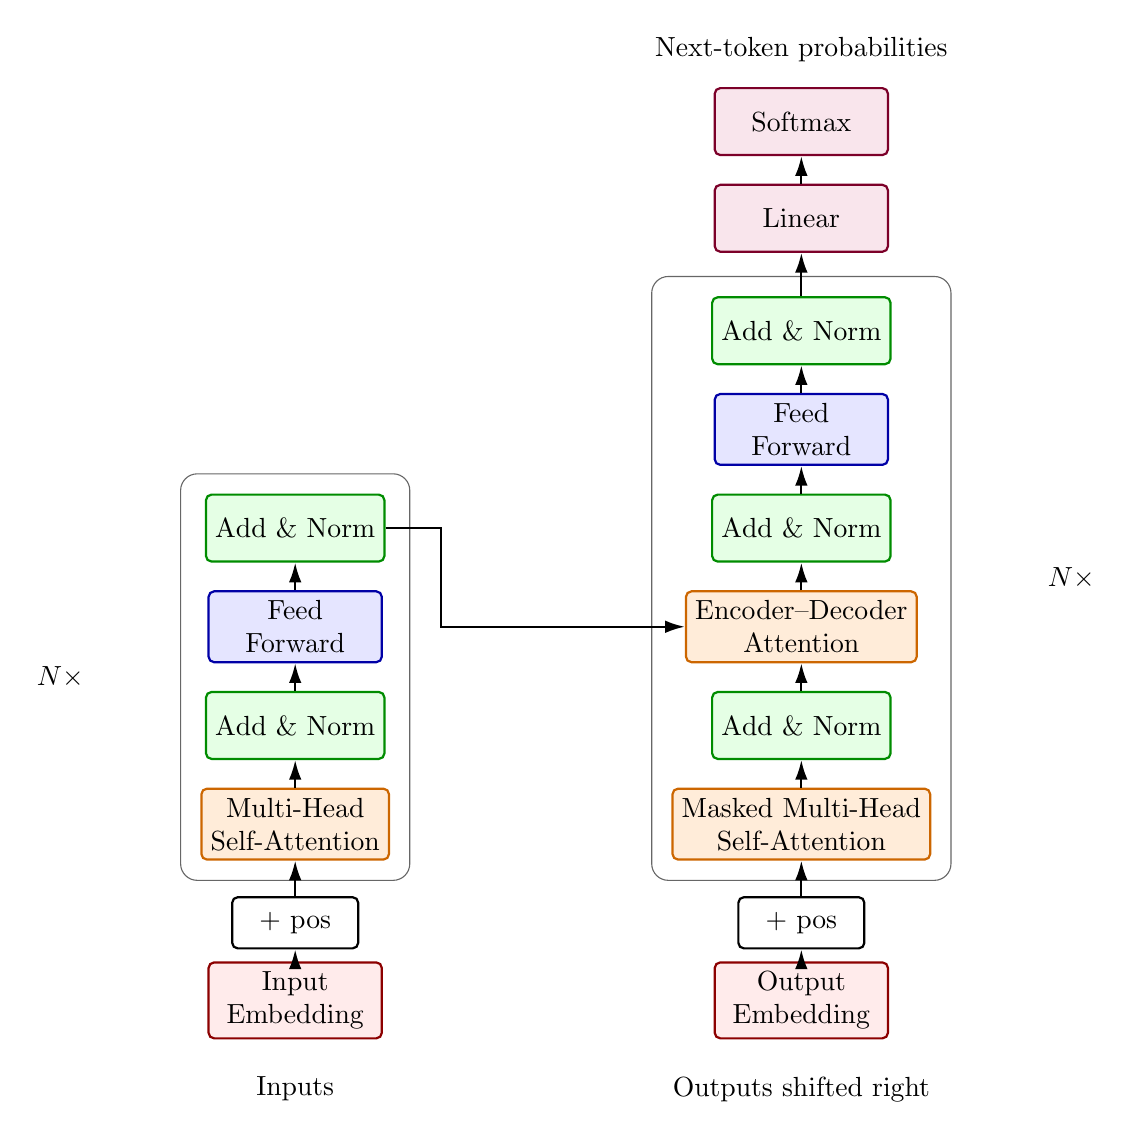
\begin{tikzpicture}[node distance=0.35cm and 1.1cm, every node/.style={transform shape}]
  % Encoder stack
  \node[emb] (inemb) {Input\\Embedding};
  \node[smallbox, above=0.15cm of inemb] (inplus) {$+$ pos};
  \node[attn, above=0.45cm of inplus] (eattn) {Multi-Head\\Self-Attention};
  \node[norm, above=0.35cm of eattn] (ean) {Add \& Norm};
  \node[mlp, above=0.35cm of ean] (eff) {Feed\\Forward};
  \node[norm, above=0.35cm of eff] (ean2) {Add \& Norm};
  \node[draw=black!60, rounded corners=6pt, fit=(eattn)(ean)(eff)(ean2), inner sep=0.25cm, label={[xshift=-1.1cm]left:$N\times$}] (encfit) {};

  % Decoder stack
  \node[emb, right=4.2cm of inemb] (outemb) {Output\\Embedding};
  \node[smallbox, above=0.15cm of outemb] (outplus) {$+$ pos};
  \node[attn, above=0.45cm of outplus] (dattn1) {Masked Multi-Head\\Self-Attention};
  \node[norm, above=0.35cm of dattn1] (dan1) {Add \& Norm};
  \node[attn, above=0.35cm of dan1] (cross) {Encoder--Decoder\\Attention};
  \node[norm, above=0.35cm of cross] (dan2) {Add \& Norm};
  \node[mlp, above=0.35cm of dan2] (dff) {Feed\\Forward};
  \node[norm, above=0.35cm of dff] (dan3) {Add \& Norm};
  \node[draw=black!60, rounded corners=6pt, fit=(dattn1)(dan1)(cross)(dan2)(dff)(dan3), inner sep=0.25cm, label={[xshift=1.1cm]right:$N\times$}] (decfit) {};

  \node[outbox, above=0.55cm of dan3] (linear) {Linear};
  \node[outbox, above=0.35cm of linear] (softmax) {Softmax};

  % arrows
  \draw[arrow] (inemb) -- (inplus);
  \draw[arrow] (inplus) -- (eattn);
  \draw[arrow] (eattn) -- (ean);
  \draw[arrow] (ean) -- (eff);
  \draw[arrow] (eff) -- (ean2);

  \draw[arrow] (outemb) -- (outplus);
  \draw[arrow] (outplus) -- (dattn1);
  \draw[arrow] (dattn1) -- (dan1);
  \draw[arrow] (dan1) -- (cross);
  \draw[arrow] (cross) -- (dan2);
  \draw[arrow] (dan2) -- (dff);
  \draw[arrow] (dff) -- (dan3);
  \draw[arrow] (dan3) -- (linear);
  \draw[arrow] (linear) -- (softmax);
  \draw[arrow] (ean2.east) -- ++(0.7,0) |- (cross.west);

  \node[below=0.35cm of inemb] {Inputs};
  \node[below=0.35cm of outemb] {Outputs shifted right};
  \node[above=0.2cm of softmax] {Next-token probabilities};
\end{tikzpicture}%
}
\end{frame}

\section{microGPT}

\begin{frame}{microGPT: the Minimal Educational GPT}
\begin{block}{What it is}
microGPT is a tiny, dependency-free Python implementation of a decoder-only GPT. It is designed to expose the complete training and inference algorithm rather than maximize efficiency.
\end{block}
\begin{itemize}
  \item Character-level language model on names.
  \item One Transformer layer in the example code: \(L=1\).
  \item Model width \(d=16\), number of heads \(H=4\), head size \(d_h=4\).
  \item Uses \textbf{RMSNorm} and a two-layer MLP \(W_2\operatorname{ReLU}(W_1x)\).
  \item Uses a learned token embedding \(E_{\text{tok}}\) and learned positional embedding \(E_{\text{pos}}\).
\end{itemize}
\end{frame}

\begin{frame}{microGPT Architecture}
\centering
\resizebox{!}{0.70\textheight}{%
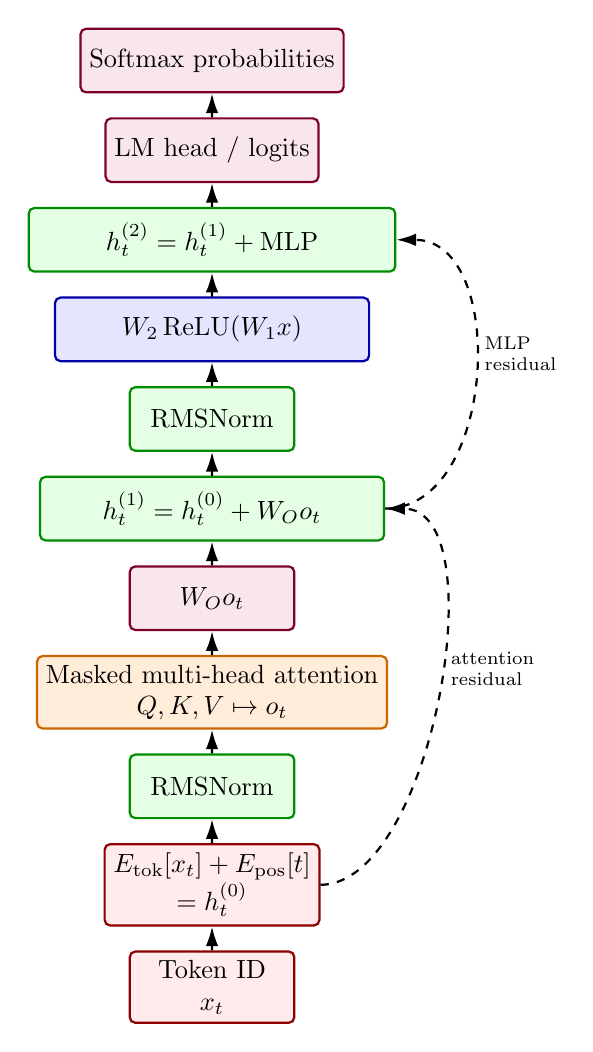
\begin{tikzpicture}[node distance=0.32cm, scale=0.95, every node/.style={transform shape}]
  \node[emb] (tok) {Token ID \\ \(x_t\)};
  \node[emb, above=of tok] (emb) {$E_{\text{tok}}[x_t] + E_{\text{pos}}[t]$\\$= h_t^{(0)}$};
  \node[norm, above=of emb] (r1) {RMSNorm};
  \node[attn, above=of r1, minimum width=4.2cm] (attn) {Masked multi-head attention\\$Q,K,V \mapsto o_t$};
  \node[outbox, above=of attn] (wo) {$W_O o_t$};
  \node[norm, above=of wo, minimum width=4.6cm] (res1) {$h_t^{(1)} = h_t^{(0)} + W_O o_t$};
  \node[norm, above=of res1] (r2) {RMSNorm};
  \node[mlp, above=of r2, minimum width=4.2cm] (mlp) {$W_2\,\mathrm{ReLU}(W_1x)$};
  \node[norm, above=of mlp, minimum width=4.9cm] (res2) {$h_t^{(2)} = h_t^{(1)} + \mathrm{MLP}$};
  \node[outbox, above=of res2] (lm) {LM head / logits};
  \node[outbox, above=of lm] (prob) {Softmax probabilities};

  \foreach \a/\b in {tok/emb,emb/r1,r1/attn,attn/wo,wo/res1,res1/r2,r2/mlp,mlp/res2,res2/lm,lm/prob}
    \draw[arrow] (\a) -- (\b);

  \draw[dashedarrow] (emb.east) .. controls +(1.5,0) and +(1.5,0) .. node[pos=0.55,right,font=\scriptsize,align=left]{attention\\residual} (res1.east);
  \draw[dashedarrow] (res1.east) .. controls +(1.5,0) and +(1.5,0) .. node[pos=0.55,right,font=\scriptsize,align=left]{MLP\\residual} (res2.east);
\end{tikzpicture}%
}
\end{frame}

\section{GPT-1}

\begin{frame}{GPT-1: Generative Pre-Training}
\begin{columns}[T,totalwidth=\textwidth]
\begin{column}{0.58\textwidth}
\begin{itemize}
  \item Introduced in \emph{Improving Language Understanding by Generative Pre-Training} (2018)~\cite{radford2018gpt}.
  \item Decoder-only Transformer adapted from the original Transformer by discarding the encoder and cross-attention.
  \item Pretraining objective:
  \[
  P(x_1,\ldots,x_T)=\prod_{t=1}^{T} P(x_t\mid x_{<t}).
  \]
  \item Fine-tuning attaches task-specific heads after generative pretraining.
\end{itemize}
\end{column}
\begin{column}{0.38\textwidth}
\begin{block}{Typical GPT-1 configuration}
\centering
\begin{tabular}{@{}ll@{}}
\toprule
Layers & 12 \\
Heads & 12 \\
Hidden size & 768 \\
Context & 512 \\
\bottomrule
\end{tabular}
\end{block}
\end{column}
\end{columns}
\end{frame}

\begin{frame}{GPT-1 Architecture}
\centering
\resizebox{!}{0.70\textheight}{%
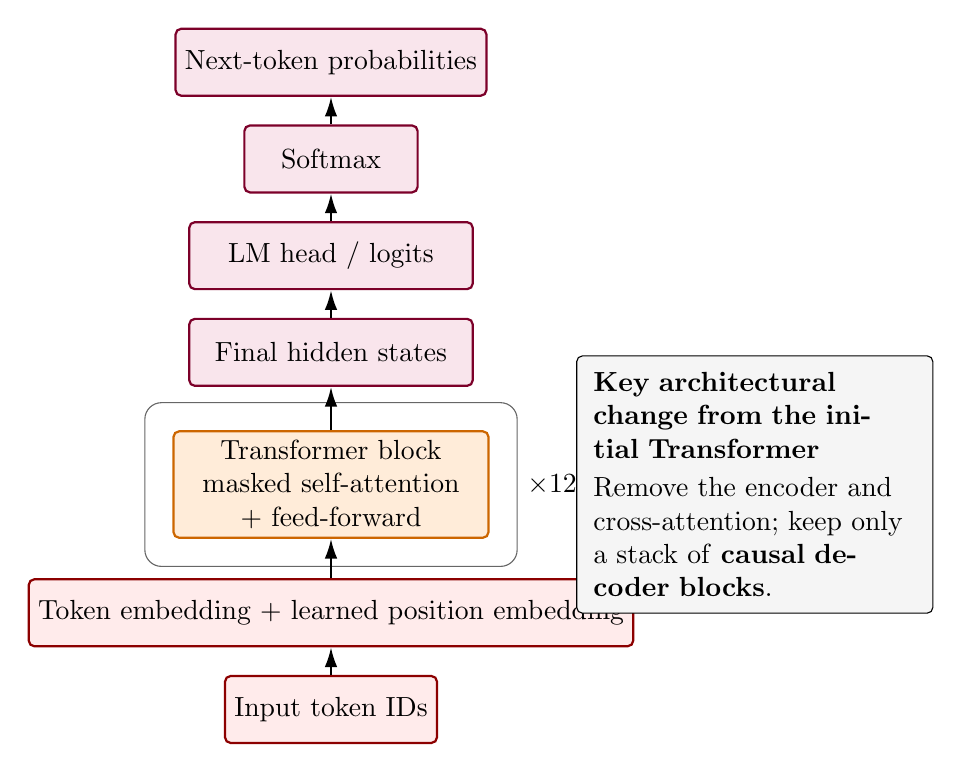
\begin{tikzpicture}[node distance=0.35cm, every node/.style={transform shape}]
  \node[emb] (inp) {Input token IDs};
  \node[emb, above=of inp, minimum width=4.2cm] (embed) {Token embedding $+$ learned position embedding};
  \node[attn, above=0.5cm of embed, minimum width=4.0cm] (block) {Transformer block\\masked self-attention\\$+$ feed-forward};
  \node[draw=black!60, rounded corners=6pt, fit=(block), inner sep=0.35cm, label=right:$\times 12$] (stack) {};
  \node[outbox, above=0.55cm of block, minimum width=3.6cm] (hid) {Final hidden states};
  \node[outbox, above=0.35cm of hid, minimum width=3.6cm] (head) {LM head / logits};
  \node[outbox, above=0.35cm of head] (sm) {Softmax};
  \node[outbox, above=0.35cm of sm] (next) {Next-token probabilities};
  \foreach \a/\b in {inp/embed,embed/block,block/hid,hid/head,head/sm,sm/next}
    \draw[arrow] (\a) -- (\b);

  \node[info, right=1.1cm of block, text width=4.1cm] {
  \textbf{Key architectural change from the initial Transformer}\par
  \vspace{0.2em}
  Remove the encoder and cross-attention; keep only a stack of \textbf{causal decoder blocks}.};
\end{tikzpicture}%
}
\end{frame}

\section{GPT-2}

\begin{frame}{GPT-2: Scaling the Decoder-Only GPT}
\begin{block}{Main message}
GPT-2 kept the same basic decoder-only architecture as GPT-1, but scaled model size, dataset size, and context handling enough to demonstrate strong zero-shot and multitask behavior~\cite{radford2019gpt2}.
\end{block}
\begin{itemize}
  \item Same core pattern: token embeddings \(\to\) stack of masked self-attention blocks \(\to\) LM head.
  \item Larger context length: 1024 tokens.
  \item Largest published model in the paper: about 1.5B parameters.
  \item Emphasis shifted from ``pretrain then fine-tune'' toward ``pretrain and prompt/use directly.''
\end{itemize}
\end{frame}

\begin{frame}{GPT-2 as an Enlarged GPT-1}
\centering
\resizebox{!}{0.70\textheight}{%
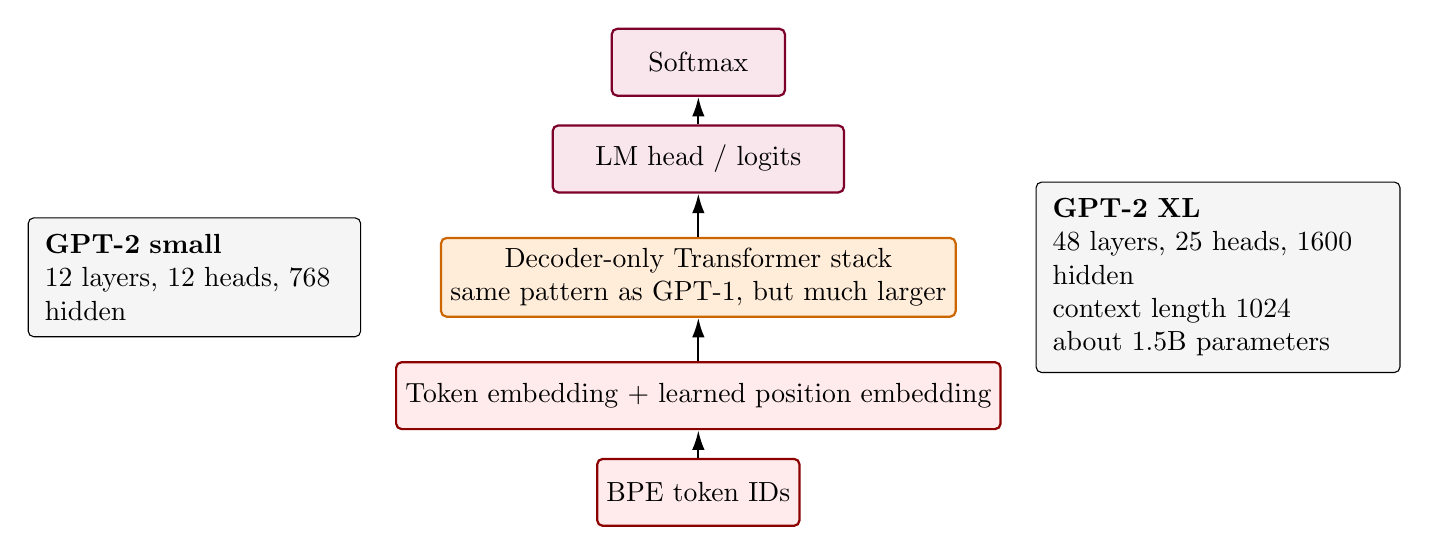
\begin{tikzpicture}[node distance=0.35cm, every node/.style={transform shape}]
  \node[emb] (inp) {BPE token IDs};
  \node[emb, above=of inp, minimum width=4.3cm] (embed) {Token embedding $+$ learned position embedding};
  \node[attn, above=0.55cm of embed, minimum width=4.1cm, minimum height=1.0cm] (stack) {Decoder-only Transformer stack\\same pattern as GPT-1, but much larger};
  \node[outbox, above=0.55cm of stack, minimum width=3.7cm] (head) {LM head / logits};
  \node[outbox, above=0.35cm of head] (sm) {Softmax};
  \foreach \a/\b in {inp/embed,embed/stack,stack/head,head/sm}
    \draw[arrow] (\a) -- (\b);

  \node[info, left=1.0cm of stack, text width=3.8cm] {
  \textbf{GPT-2 small}\par 12 layers, 12 heads, 768 hidden};
  \node[info, right=1.0cm of stack, text width=4.2cm] {
  \textbf{GPT-2 XL}\par 48 layers, 25 heads, 1600 hidden\par context length 1024\par about 1.5B parameters};
\end{tikzpicture}%
}
\end{frame}

\section{GPT-3}

\begin{frame}{GPT-3: Scaling to Few-Shot Learning}
\begin{block}{Main message}
GPT-3 again retained the decoder-only Transformer pattern, but scaled it drastically~\cite{brown2020gpt3}. The headline result was strong \textbf{in-context learning}: the model can perform new tasks from prompts alone, with zero, one, or a few demonstrations.
\end{block}
\begin{itemize}
  \item Decoder-only Transformer with causal self-attention.
  \item Context length in the original paper: 2048 tokens.
  \item Largest model: 175B parameters.
  \item Major conceptual shift: prompting becomes a central interface to behavior.
\end{itemize}
\end{frame}

\begin{frame}{GPT-3 Architecture: Same Skeleton, Much Larger Scale}
\centering
\resizebox{!}{0.70\textheight}{%
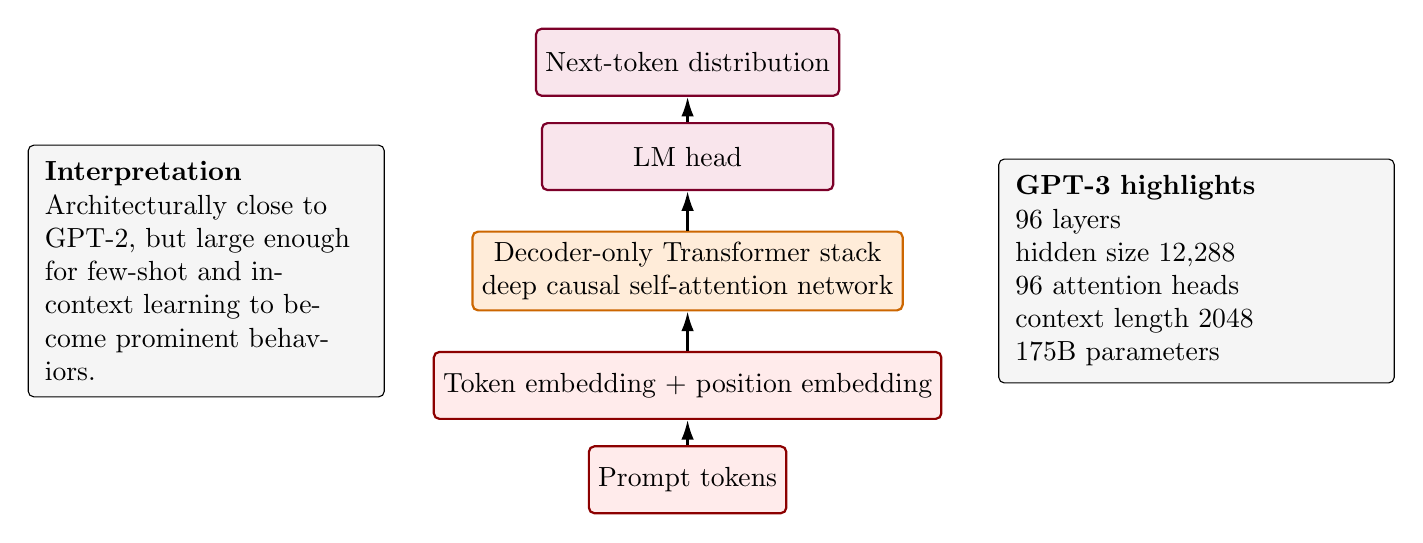
\begin{tikzpicture}[node distance=0.32cm, every node/.style={transform shape}]
  \node[emb] (inp) {Prompt tokens};
  \node[emb, above=of inp, minimum width=4.5cm] (embed) {Token embedding $+$ position embedding};
  \node[attn, above=0.5cm of embed, minimum width=4.3cm, minimum height=1.0cm] (stack) {Decoder-only Transformer stack\\deep causal self-attention network};
  \node[outbox, above=0.5cm of stack, minimum width=3.7cm] (head) {LM head};
  \node[outbox, above=0.32cm of head] (next) {Next-token distribution};
  \foreach \a/\b in {inp/embed,embed/stack,stack/head,head/next}
    \draw[arrow] (\a) -- (\b);

  \node[info, right=1.2cm of stack, text width=4.6cm] {
  \textbf{GPT-3 highlights}\par
  96 layers\par
  hidden size 12,288\par
  96 attention heads\par
  context length 2048\par
  175B parameters};

  \node[info, left=1.1cm of stack, text width=4.1cm] {
  \textbf{Interpretation}\par
  Architecturally close to GPT-2, but large enough for few-shot and in-context learning to become prominent behaviors.};
\end{tikzpicture}%
}
\end{frame}

\section{Evolution Summary}


\begin{frame}{Architecture Evolution at a Glance}
\scriptsize
\centering
\renewcommand{\arraystretch}{1.18}
\begin{tabular}{p{1.9cm} p{2.35cm} p{2.55cm} p{2.35cm} p{2.75cm}}
\toprule
\textbf{Model} & \textbf{Core architecture} & \textbf{Objective} & \textbf{Scale} & \textbf{Shift} \\
\midrule
Initial Transformer & Encoder--decoder & Sequence-to-sequence & 6 encoder + 6 decoder layers & Attention replaces recurrence \\
microGPT & Tiny decoder-only GPT & Character-level next-token prediction & 1 layer, $d=16$, 4 heads & Minimal educational implementation \\
GPT-1 & Decoder-only Transformer & Generative pretraining + fine-tuning & 12 layers, $d=768$ & Transfer via pretraining \\
GPT-2 & Larger decoder-only Transformer & Large-scale next-token prediction & Up to 1.5B params & Zero-shot behavior emerges \\
GPT-3 & Much larger decoder-only Transformer & Massive next-token prediction & 175B params & Few-shot / in-context learning \\
\bottomrule
\end{tabular}
\vspace{0.4em}

\footnotesize References: Vaswani et al. (2017), Radford et al. (2018, 2019), Brown et al. (2020).
\end{frame}


\begin{frame}{The Main Structural Trend}
\begin{block}{From the initial Transformer to GPT-3}
\centering
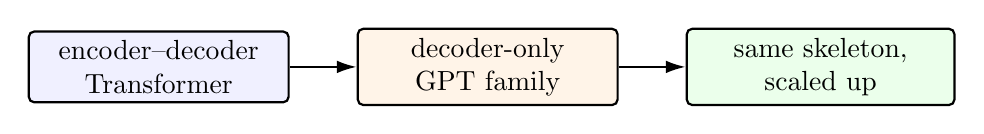
\begin{tikzpicture}[node distance=0.85cm]
\node[box, fill=blue!6, minimum width=3.3cm] (a) {encoder--decoder\\Transformer};
\node[box, fill=orange!9, right=of a, minimum width=3.3cm] (b) {decoder-only\\GPT family};
\node[box, fill=green!8, right=of b, minimum width=3.4cm] (c) {same skeleton,\\scaled up};
\draw[arrow] (a)--(b);
\draw[arrow] (b)--(c);
\end{tikzpicture}
\end{block}
\begin{itemize}
  \item The original Transformer introduced the attention-based architecture.
  \item GPT keeps only the causal decoder side.
  \item microGPT strips that architecture down to its essentials.
  \item GPT-1, GPT-2, and GPT-3 mostly differ by \textbf{scale}, training data, and behavior induced by scale.
\end{itemize}
\end{frame}


\section{References}

\begin{frame}[allowframebreaks]{References}
\tiny
\begin{thebibliography}{99}

\bibitem[Vaswani et al., 2017]{vaswani2017attention}
Ashish Vaswani, Noam Shazeer, Niki Parmar, Jakob Uszkoreit, Llion Jones, Aidan N. Gomez, Lukasz Kaiser, and Illia Polosukhin.
\newblock \emph{Attention Is All You Need}.
\newblock arXiv:1706.03762, 2017.
\newblock \url{https://arxiv.org/abs/1706.03762}

\bibitem[Radford et al., 2018]{radford2018gpt}
Alec Radford, Karthik Narasimhan, Tim Salimans, and Ilya Sutskever.
\newblock \emph{Improving Language Understanding by Generative Pre-Training}.
\newblock OpenAI technical report, 2018.
\newblock \url{https://cdn.openai.com/research-covers/language-unsupervised/language_understanding_paper.pdf}

\bibitem[Radford et al., 2019]{radford2019gpt2}
Alec Radford, Jeffrey Wu, Rewon Child, David Luan, Dario Amodei, and Ilya Sutskever.
\newblock \emph{Language Models are Unsupervised Multitask Learners}.
\newblock OpenAI technical report, 2019.
\newblock \url{https://cdn.openai.com/better-language-models/language_models_are_unsupervised_multitask_learners.pdf}

\bibitem[Brown et al., 2020]{brown2020gpt3}
Tom B. Brown et al.
\newblock \emph{Language Models are Few-Shot Learners}.
\newblock arXiv:2005.14165, 2020.
\newblock \url{https://arxiv.org/abs/2005.14165}

\bibitem[Karpathy, microGPT code]{karpathyMicroGPT}
Andrej Karpathy.
\newblock Minimal GPT-style educational code used as the microGPT reference in these slides.
\newblock User-provided code snippet in this study session.

\end{thebibliography}
\end{frame}

\begin{frame}{End}
\centering
{\Large LLM Architecture Evolution}\par
\bigskip
{\large From the initial Transformer to GPT-3}\par
\bigskip\bigskip
Questions?
\end{frame}

\end{document}
